\documentclass[11pt]{article}
\usepackage[a4paper,margin=1in]{geometry}
\usepackage{amsmath,amssymb,amsfonts}
\usepackage{booktabs}
\usepackage{graphicx}
\usepackage{caption}
\usepackage{enumitem}
\usepackage[hidelinks]{hyperref}
\usepackage{xurl}
\usepackage{microtype}
\usepackage{array}
\usepackage[table]{xcolor}

\title{2D Single-Target Window-Measure Note\\\large The Difference Between Occupancy Share and Ever-Visit Probability}
\author{}
\date{}

\setlist{nosep}
\setlength{\textfloatsep}{8pt plus 2pt minus 2pt}
\setlength{\floatsep}{6pt plus 2pt minus 2pt}
\setlength{\intextsep}{6pt plus 2pt minus 2pt}
\setlength{\abovecaptionskip}{4pt}
\setlength{\belowcaptionskip}{0pt}
\setlength{\tabcolsep}{5pt}
\renewcommand{\arraystretch}{1.10}

\begin{document}
\maketitle

\section*{Main Point}
This note now uses a milder corridor-only variant to explain the same question: why \texttt{target funnel} is not at $100\%$, even though every trajectory must eventually pass through it.

The answer has two parts:
\begin{enumerate}
  \item The current figure shows \textbf{window-conditioned occupancy share}: how much pre-hit time is spent in each region.
  \item The intuitive statement ``every trajectory must pass the funnel'' corresponds to \textbf{ever-visit probability}: whether the trajectory ever enters that region before absorption.
\end{enumerate}
Both are correct, but they are different observables and therefore need not have the same numerical values.

\section{Geometry and Spatial Partition}
We keep the same symmetric one-target geometry from \texttt{grid2d\_one\_two\_target\_gating}, but switch to a milder corridor-only soft-bias variant:
\[
L_x=60,\qquad W_y=15,\qquad (x_s,y_s)=(7,7),\qquad (x_t,y_t)=(58,7).
\]
The corridor band is $y=5,\dots,9$. The two semipermeable membranes sit on the upper and lower interfaces between the corridor and the outer reservoir, and the membrane span is $x=5,\dots,54$. In this explainer we do not draw the gate contour; we keep only the spatial partition. To make the color-to-region mapping immediately readable, both main figures below repeat the same partition schematic directly above the corresponding plot instead of forcing the reader to look back.

The corridor-related dynamical parameters of this baseline are also fixed and should be stated explicitly:
\begin{itemize}
  \item the corridor half-width is $2$, so the midline is $y=7$ and the corridor is exactly $y=5,\dots,9$;
  \item the wall margin is $5$, so the semipermeable membranes only cover $x=5,\dots,54$, i.e. the interface edges $(x,4)\leftrightarrow(x,5)$ and $(x,9)\leftrightarrow(x,10)$;
  \item every corridor site carries a \textbf{local eastward bias}, with direction \texttt{E};
  \item inside the membrane span, namely for $5 \le x \le 54$, the local bias strength is reduced to $\delta_{\mathrm{core}}=0.8$;
  \item in the left and right corridor openings, namely for $x<5$ or $x>54$, the local bias strength is $\delta_{\mathrm{open}}=0.0$, so the openings no longer receive any extra rightward push;
  \item the upper and lower outer reservoirs already had no local rightward bias; after this change, the only sites with local rightward driving are the main corridor cells $5 \le x \le 54,\ 5 \le y \le 9$;
  \item the variant still includes a \textbf{global leftward bias} $(b_x,0)=(-0.08,0)$, so outside the main corridor segment the dynamics reduce to that weaker leftward background drift;
  \item the symmetric membrane permeabilities are $kappa_{c\to o}=kappa_{o\to c}=0.002$;
  \item the laziness parameter used in the transition construction is $q=0.8$.
\end{itemize}
One subtle but important point is that the main-corridor local bias points to the \emph{right}, whereas the global bias points to the \emph{left}; the bimodal structure is produced by the competition between these two driving layers together with the membrane bottleneck. We also ran an exact scan with $\delta_{\mathrm{open}}=0$: once $\delta_{\mathrm{core}}\le 0.6$ the two-peak structure collapses, while $\delta_{\mathrm{core}}=0.8$ is a reasonable compromise between ``not too hard'' and ``still visibly bimodal''.

\section{How Peak1, Valley, and Peak2 Are Defined}
These names are not chosen by eye. They come from the repo-native exact rules.

\subsection{Step 1: detect two credible peaks}
Given the total first-passage pmf $f(t)$, the code first builds a smoothed envelope with window length $7$, then calls \texttt{find\_two\_peaks} to detect two credible local peaks. The routine does not merely ask for local maxima. It also requires:
\begin{itemize}
  \item each peak height to be at least $6\%$ of the global maximum;
  \item a minimum separation of $20$ time steps between the two peaks;
  \item a genuine valley between the peaks rather than a shoulder;
  \item no extreme peak imbalance;
  \item a visible valley drop relative to the peak heights.
\end{itemize}
So \texttt{peak1} and \texttt{peak2} are the two peak locations that survive this credibility filter.

\subsection{Step 2: define the valley between them}
Once two credible peaks are found, the code takes the minimum of the smoothed curve between them:
\[
t_{\mathrm{valley}}=\arg\min_{t\in[t_{\mathrm{peak1}},\,t_{\mathrm{peak2}}]} f_s(t),
\]
where $f_s$ denotes the smoothed curve. Hence:
\begin{itemize}
  \item the center of \texttt{peak1} is $t_{\mathrm{peak1}}$;
  \item the center of \texttt{valley} is $t_{\mathrm{valley}}$;
  \item the center of \texttt{peak2} is $t_{\mathrm{peak2}}$.
\end{itemize}

\subsection{Step 3: choose a shared window half-width}
The windows are not hand-tuned. Their common half-width is
\[
\mathrm{half}=\max\!\left(8,\ \min\!\left(26,\ \left\lfloor\frac{t_{\mathrm{peak2}}-t_{\mathrm{peak1}}}{7}\right\rfloor\right)\right).
\]
The three windows are then
\[
[t_{\mathrm{peak1}}-\mathrm{half},\ t_{\mathrm{peak1}}+\mathrm{half}],
\quad
[t_{\mathrm{valley}}-\mathrm{half},\ t_{\mathrm{valley}}+\mathrm{half}],
\quad
[t_{\mathrm{peak2}}-\mathrm{half},\ t_{\mathrm{peak2}}+\mathrm{half}].
\]

For the current corridor-only soft variant, the exact centers are
\[
t_{\mathrm{peak1}}=554,\qquad t_{\mathrm{valley}}=1490,\qquad t_{\mathrm{peak2}}=2327.
\]
Since $t_{\mathrm{peak2}}-t_{\mathrm{peak1}}=1773$, this still yields $\mathrm{half}=26$, so the actual windows used in this report are
\[
\texttt{peak1}=[528,580],\qquad
\texttt{valley}=[1464,1516],\qquad
\texttt{peak2}=[2301,2353].
\]

\subsection{Relation to the phase criterion}
The window definition is not the same thing as the clear-double-peak phase criterion. The windows only define three representative time ranges. The phase test separately checks whether the two peaks are truly separated. In the canonical one-target rule:
\begin{itemize}
  \item \texttt{find\_two\_peaks} must identify two credible peaks;
  \item the separation score must satisfy \(\mathrm{sep}_{\mathrm{peaks}}\ge 1\) for a case to count as a clear double peak.
\end{itemize}
For the present soft-bias variant we obtain \(\mathrm{sep}_{\mathrm{peaks}}\approx 0.675\). So the case still has two credible peaks, but it no longer qualifies as a \emph{clear} double peak under the repo-native threshold; in phase language it is \texttt{phase=1} rather than \texttt{phase=2}.

\section{What the Current Figure Actually Measures}
\subsection{Window-conditioned occupancy share}
Let $X_t$ be the position at time $t$, let $T$ be the first-passage time, and let $W$ be one of the windows \texttt{peak1}, \texttt{valley}, or \texttt{peak2}. For any region $R$, the main quantity shown in the current figure is
\[
p^{\mathrm{occ}}_W(R)
=
\frac{
\mathbb{E}\!\left[
\mathbf{1}_{\{T\in W\}}
\sum_{t=0}^{T-1}\mathbf{1}_{\{X_t\in R\}}
\right]
}{
\mathbb{E}\!\left[
\mathbf{1}_{\{T\in W\}}\,T
\right]
}.
\]
Its meaning is:
\begin{quote}
Among trajectories that hit in window $W$, pick a random pre-hit time point; the probability that it lies in region $R$ is \(p^{\mathrm{occ}}_W(R)\).
\end{quote}

This is therefore a \textbf{time-weighted} quantity. A trajectory may be forced to pass through the funnel, but if it spends very little time there, its occupancy contribution remains small.

\subsection{Why the funnel does not automatically become $100\%$}
Consider a toy example:
\begin{itemize}
  \item every trajectory spends about $100$ steps in the corridor;
  \item then it enters the funnel and spends only $2$ steps there before absorption.
\end{itemize}
Then
\[
p^{\mathrm{visit}}(\texttt{funnel}) = 100\%,
\qquad
p^{\mathrm{occ}}(\texttt{funnel}) \approx \frac{2}{102}\approx 2\%.
\]
So ``must pass through'' does not imply ``dominates the time-weighted occupancy''.

\section{What the Intuitive Question Refers To}
\subsection{Ever-visit probability}
If instead we ask:
\begin{quote}
Among trajectories that hit in window $W$, how many ever enter region $R$ before absorption?
\end{quote}
then the relevant quantity is
\[
p^{\mathrm{visit}}_W(R)
=
\mathbb{P}\!\left(\exists t<T:\ X_t\in R \,\middle|\, T\in W\right).
\]
This is a path-event probability, not a time-occupancy fraction.

For \texttt{target funnel} in the present geometry, the exact calculation gives
\[
p^{\mathrm{visit}}_{\texttt{peak1}}(\texttt{funnel})
=
p^{\mathrm{visit}}_{\texttt{valley}}(\texttt{funnel})
=
p^{\mathrm{visit}}_{\texttt{peak2}}(\texttt{funnel})
=1.
\]
So the intuition that every trajectory must pass through the funnel is correct; it simply corresponds to \textbf{ever-visit}, not to \textbf{occupancy share}.

\section{Direct Comparison of the Two Observables}
We keep both of the following figures as main figures rather than treating one as mere supplementary material, and we place them back to back so the reading flow is not interrupted by other plots or tables. A good reading order is: first inspect Fig.~\ref{fig:overview-en} to understand where the time is spent; then move directly to Fig.~\ref{fig:profile-bars-en} to see how the ranking changes when we switch from a time-weighted observable to a path-event observable.

\begin{figure}[!htbp]
  \centering
  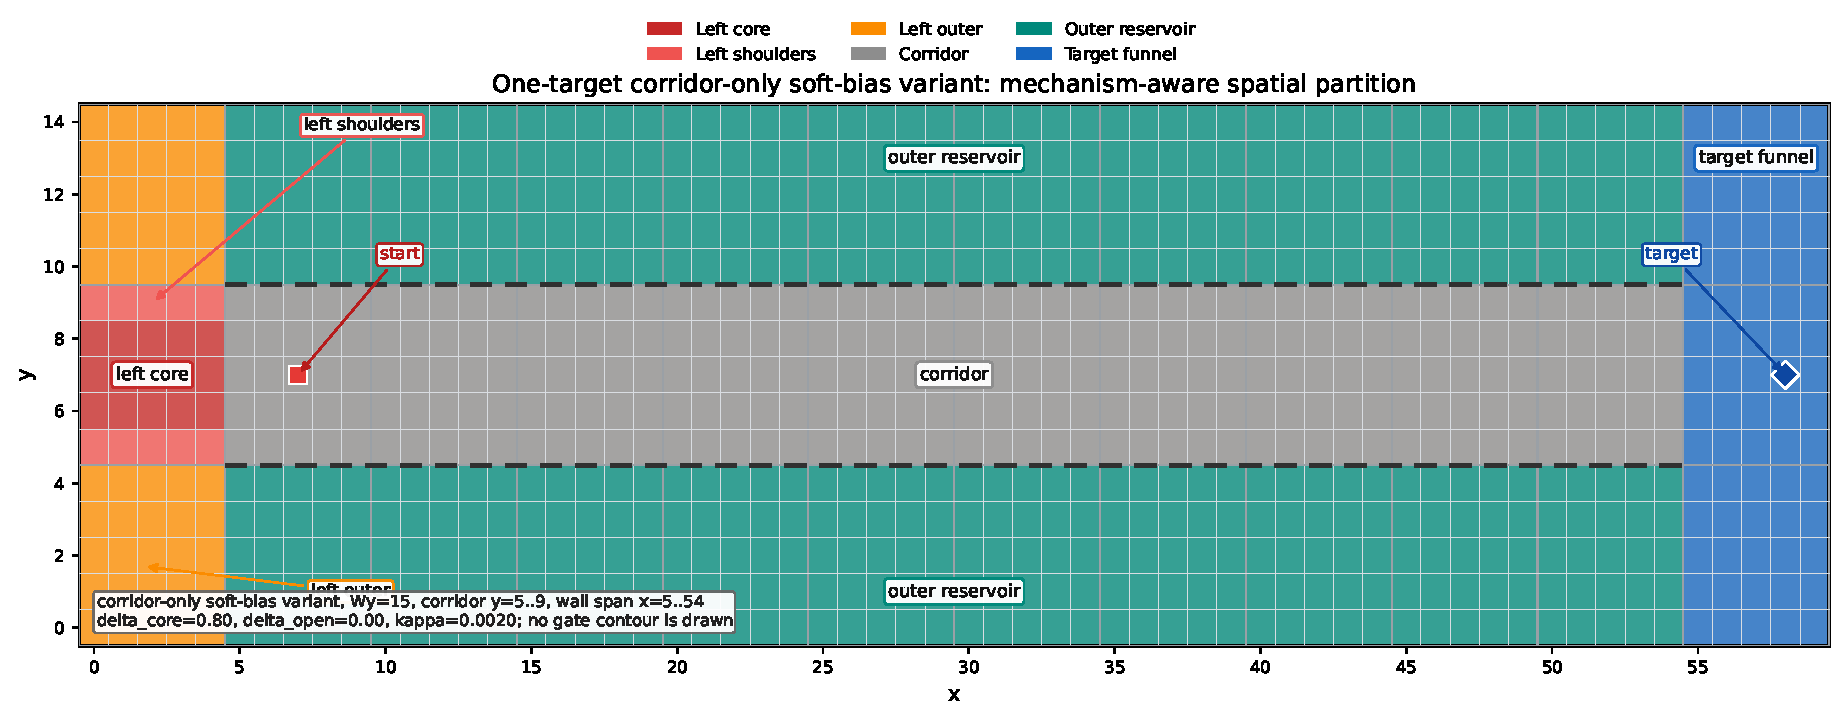
\includegraphics[width=0.92\linewidth]{../artifacts/figures/one_target_partition.pdf}

  \vspace{0.35em}
  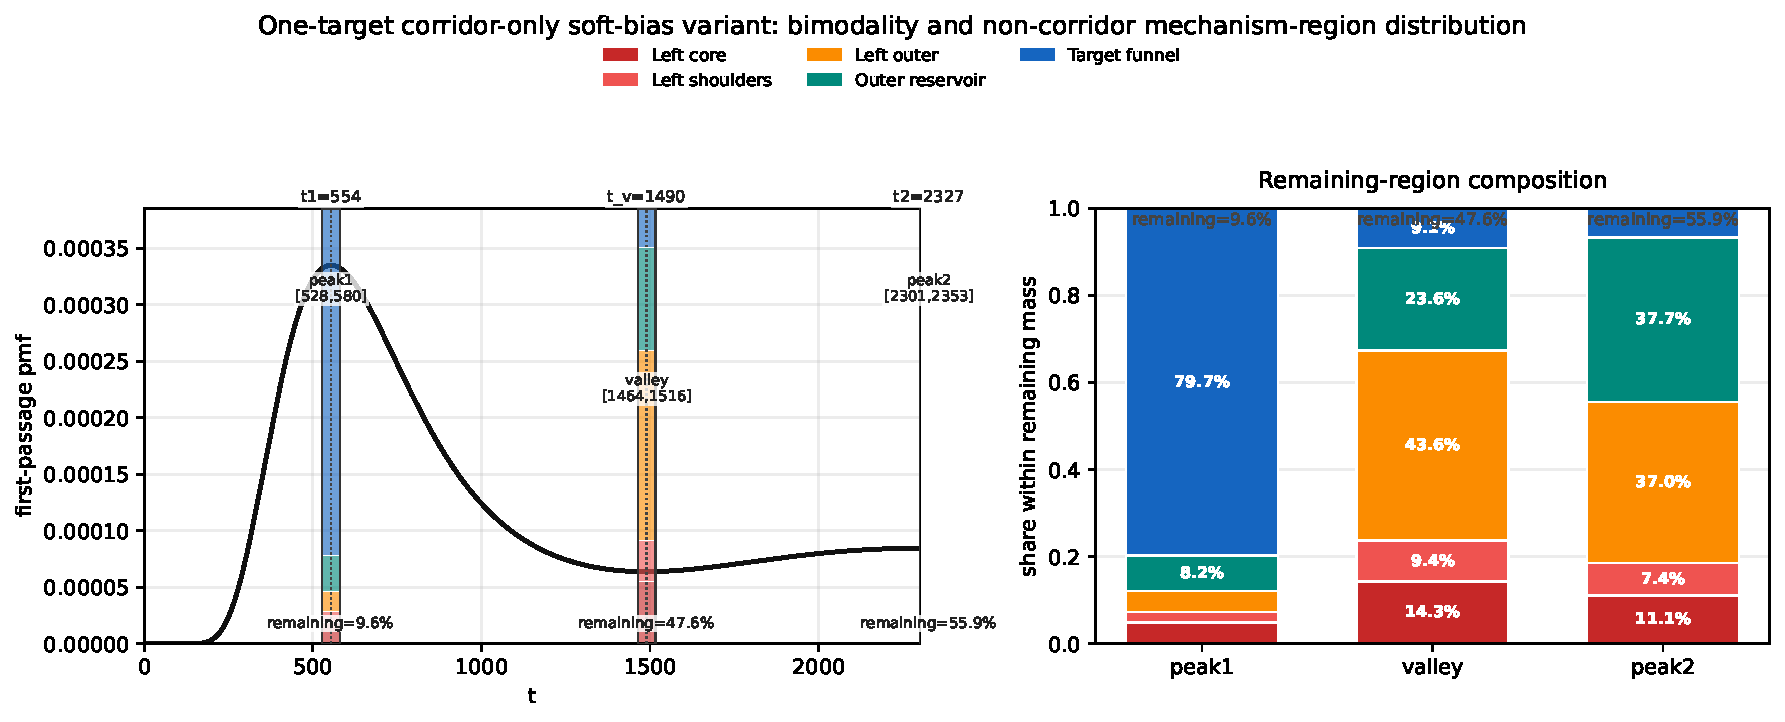
\includegraphics[width=0.98\linewidth]{../artifacts/figures/one_target_bimodal_non_corridor.pdf}
  \caption{Overview layout for the first main figure. Top: mechanism-aware spatial partition of the corridor-only soft-bias variant, with the full state space split into \texttt{left core}, \texttt{left shoulders}, \texttt{left outer}, \texttt{corridor}, \texttt{outer reservoir}, and \texttt{target funnel}. Bottom: the occupancy main figure, where full-height window-composition bars are drawn directly on top of the exact bimodal first-passage curve. The right panel shows the same non-corridor composition as standalone stacked bars. This keeps the color-to-region mapping visible right next to the figure.}
  \label{fig:overview-en}
\end{figure}

Read Fig.~\ref{fig:overview-en} first as the ``time-budget'' view: it tells us where the pre-hit time mass accumulates within the same hitting window once the corridor has been factored out.

\begin{figure}[!htbp]
  \centering
  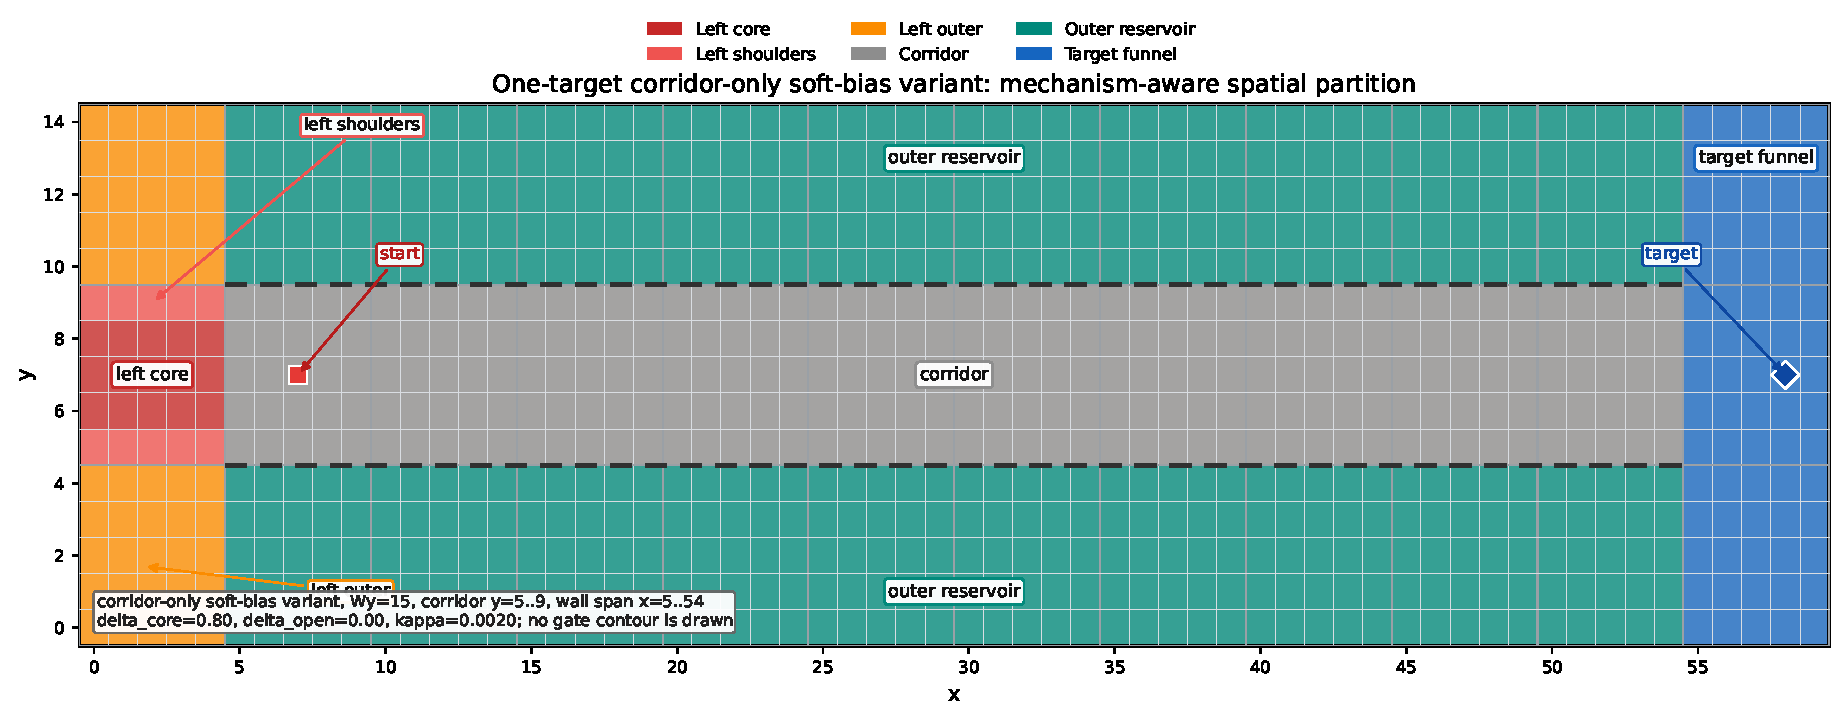
\includegraphics[width=0.92\linewidth]{../artifacts/figures/one_target_partition.pdf}

  \vspace{0.35em}
  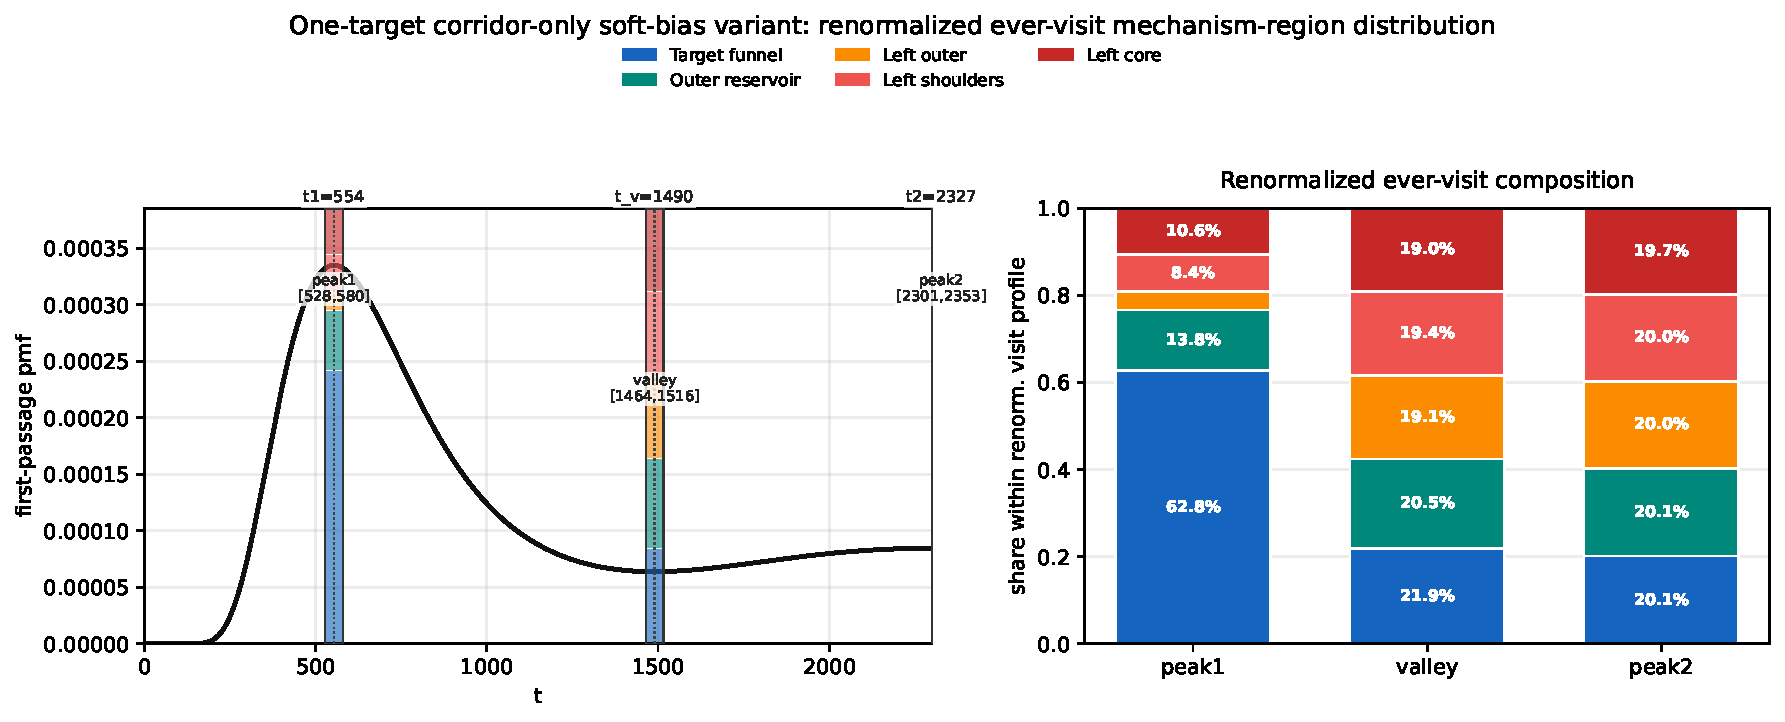
\includegraphics[width=0.98\linewidth]{../artifacts/figures/one_target_ever_visit_non_corridor.pdf}
  \caption{The second main figure uses the same overview layout, with the spatial partition placed directly above the ever-visit figure. The lower panel keeps the same exact bimodal first-passage curve and the same three windows, but replaces the regional weights by the normalized ever-visit profile. The right panel shows the renormalized ever-visit composition for each window. This is not a direct stack of raw ever-visit probabilities; the normalization is used only to make the shape comparable to the occupancy figure within the same visual grammar.}
  \label{fig:profile-bars-en}
\end{figure}

\begin{figure}[!htbp]
  \centering
  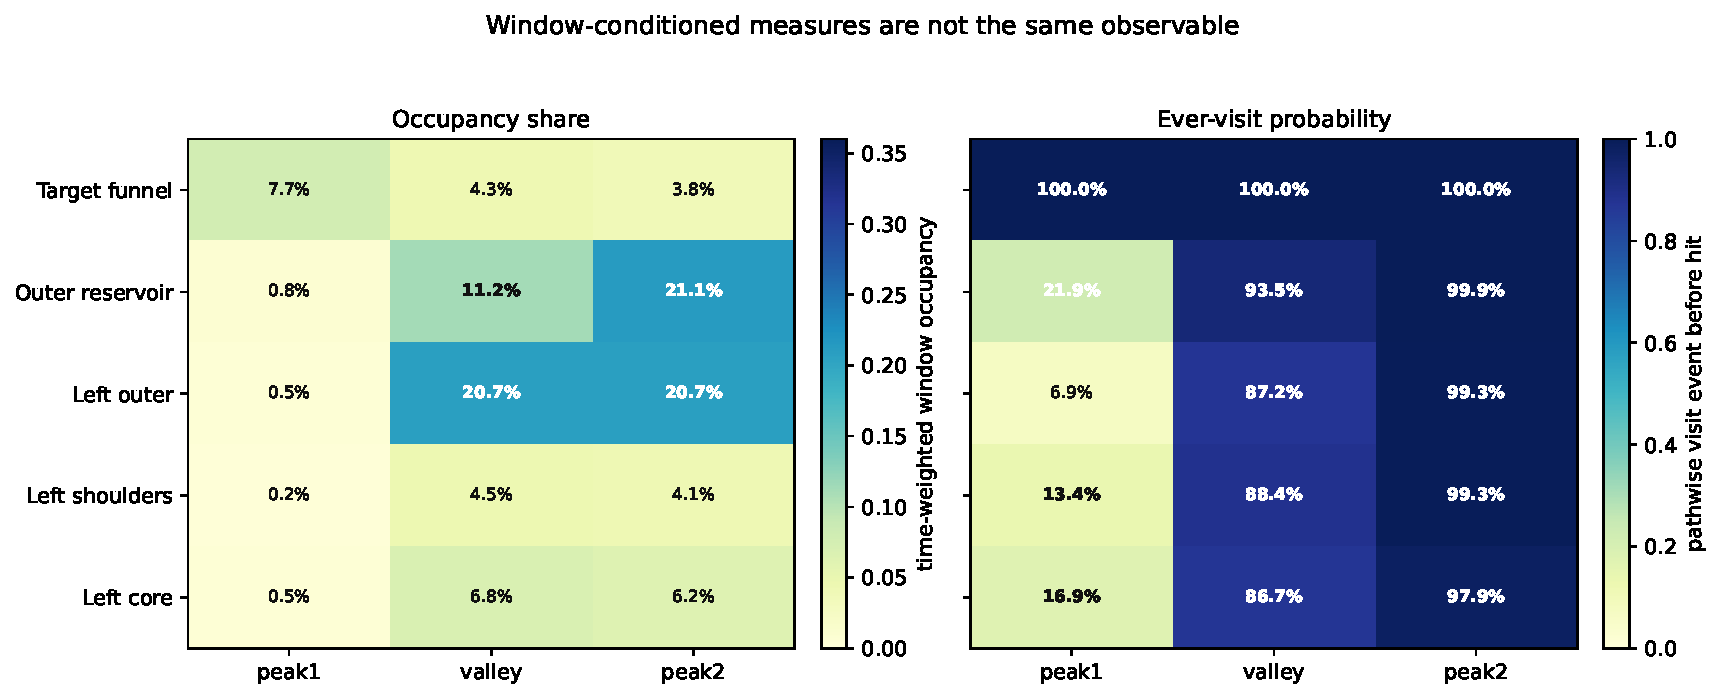
\includegraphics[width=0.92\linewidth]{../artifacts/figures/window_measure_comparison.pdf}
  \caption{Occupancy share on the left and ever-visit probability on the right. The key row is \texttt{target funnel}: its occupancy share is only about $7.7\% / 4.3\% / 3.8\%$, while its ever-visit probability is $100\%$ in all three windows. This is exactly the distinction between a time-weighted observable and a path-event observable.}
  \label{fig:measure-compare-en}
\end{figure}

\begin{table}[!htbp]
  \centering
  \footnotesize
  \begin{tabular}{lcccccc}
\toprule
Region & Occ. p1 & Visit p1 & Occ. valley & Visit valley & Occ. p2 & Visit p2 \\
\midrule
Target funnel & 7.7\% & 100.0\% & 4.3\% & 100.0\% & 3.8\% & 100.0\% \\
Outer reservoir & 0.8\% & 21.9\% & 11.2\% & 93.5\% & 21.1\% & 99.9\% \\
Left outer & 0.5\% & 6.9\% & 20.7\% & 87.2\% & 20.7\% & 99.3\% \\
Left shoulders & 0.2\% & 13.4\% & 4.5\% & 88.4\% & 4.1\% & 99.3\% \\
Left core & 0.5\% & 16.9\% & 6.8\% & 86.7\% & 6.2\% & 97.9\% \\
\bottomrule
\end{tabular}

  \caption{Exact comparison between occupancy share and ever-visit probability across the three windows.}
  \label{tab:measure-compare-en}
\end{table}

\begin{table}[!htbp]
  \centering
  \footnotesize
  \begin{tabular}{lcc}
\toprule
Window & Cosine similarity & Total variation distance \\
\midrule
peak1 & 0.9838 & 0.1728 \\
valley & 0.8270 & 0.2758 \\
peak2 & 0.8153 & 0.3461 \\
\bottomrule
\end{tabular}

  \caption{Similarity between the two normalized profiles on the same five-region basis. A cosine similarity closer to $1$ means the shapes are more alike; a smaller total-variation distance means they are closer in mass distribution.}
  \label{tab:profile-sim-en}
\end{table}

It is important that Table~\ref{tab:profile-sim-en} compares the shapes of two \emph{normalized profiles}. It does \emph{not} mean that raw ever-visit probabilities themselves form a composition. The comparison only answers whether the relative importance ordering of regions is similar across the two observables.

\section{Why Monte Carlo and Exact Computation Agree}
\subsection{If Monte Carlo estimates occupancy share}
Let the $m$-th Monte Carlo trajectory have first-passage time $T_m$ and path $(X_t^{(m)})_{t=0}^{T_m-1}$. The natural Monte Carlo estimator for occupancy share is
\[
\widehat p^{\mathrm{occ}}_W(R)
=
\frac{
\sum_{m=1}^M
\mathbf{1}_{\{T_m\in W\}}
\sum_{t=0}^{T_m-1}\mathbf{1}_{\{X_t^{(m)}\in R\}}
}{
\sum_{m=1}^M
\mathbf{1}_{\{T_m\in W\}}\,T_m
}.
\]
This is exactly ``flatten all pre-hit time points from trajectories that hit in window $W$ and count what fraction falls in $R$''. By the law of large numbers, it converges to the exact occupancy share shown in the figure.

\subsection{If Monte Carlo estimates ever-visit probability}
The corresponding estimator for ever-visit probability is
\[
\widehat p^{\mathrm{visit}}_W(R)
=
\frac{
\sum_{m=1}^M
\mathbf{1}_{\{T_m\in W\}}
\mathbf{1}_{\{\exists t<T_m:\ X_t^{(m)}\in R\}}
}{
\sum_{m=1}^M
\mathbf{1}_{\{T_m\in W\}}
}.
\]
This converges to the exact ever-visit probability, not to occupancy share.

\subsection{So when should Monte Carlo and exact results look similar?}
The answer is simple:
\begin{itemize}
  \item if Monte Carlo estimates the same observable, it should agree with the exact result up to sampling noise;
  \item if Monte Carlo estimates a different observable, it may look very different.
\end{itemize}

In the present example:
\begin{itemize}
  \item a time-point-based Monte Carlo estimate converges to occupancy share;
  \item an event-based Monte Carlo estimate gives \texttt{target funnel} close to $100\%$.
\end{itemize}

\section*{Summary}
The main purpose of this note is not to introduce a new mechanism, but to separate two observables that are often mixed together:
\begin{enumerate}
  \item \textbf{occupancy share}: time-weighted, asking where the process spends its time;
  \item \textbf{ever-visit probability}: event-based, asking whether the process ever reaches a region.
\end{enumerate}
Once the distinction is made explicit, there is no contradiction in saying that \texttt{target funnel} is a mandatory path event while still carrying only a small fraction of the time-weighted spatial distribution.

\end{document}
